\documentclass{article}
\usepackage{caption}
\usepackage{subcaption}
\usepackage{graphicx}
\usepackage{tikz}
\usepackage{tikzsymbols}
\usetikzlibrary{calc}
\usepackage{float}
\usepackage{pdflscape}
\usepackage{geometry}
\geometry{a4paper, landscape, margin=1cm}
\pagestyle{empty}

\def\centerarc[#1](#2)(#3:#4:#5){\draw[#1] ($(#2)+({#5*cos(#3)},{#5*sin(#3)})$) arc (#3:#4:#5);}

\begin{document}
	\centering
	\begin{figure}[H]
			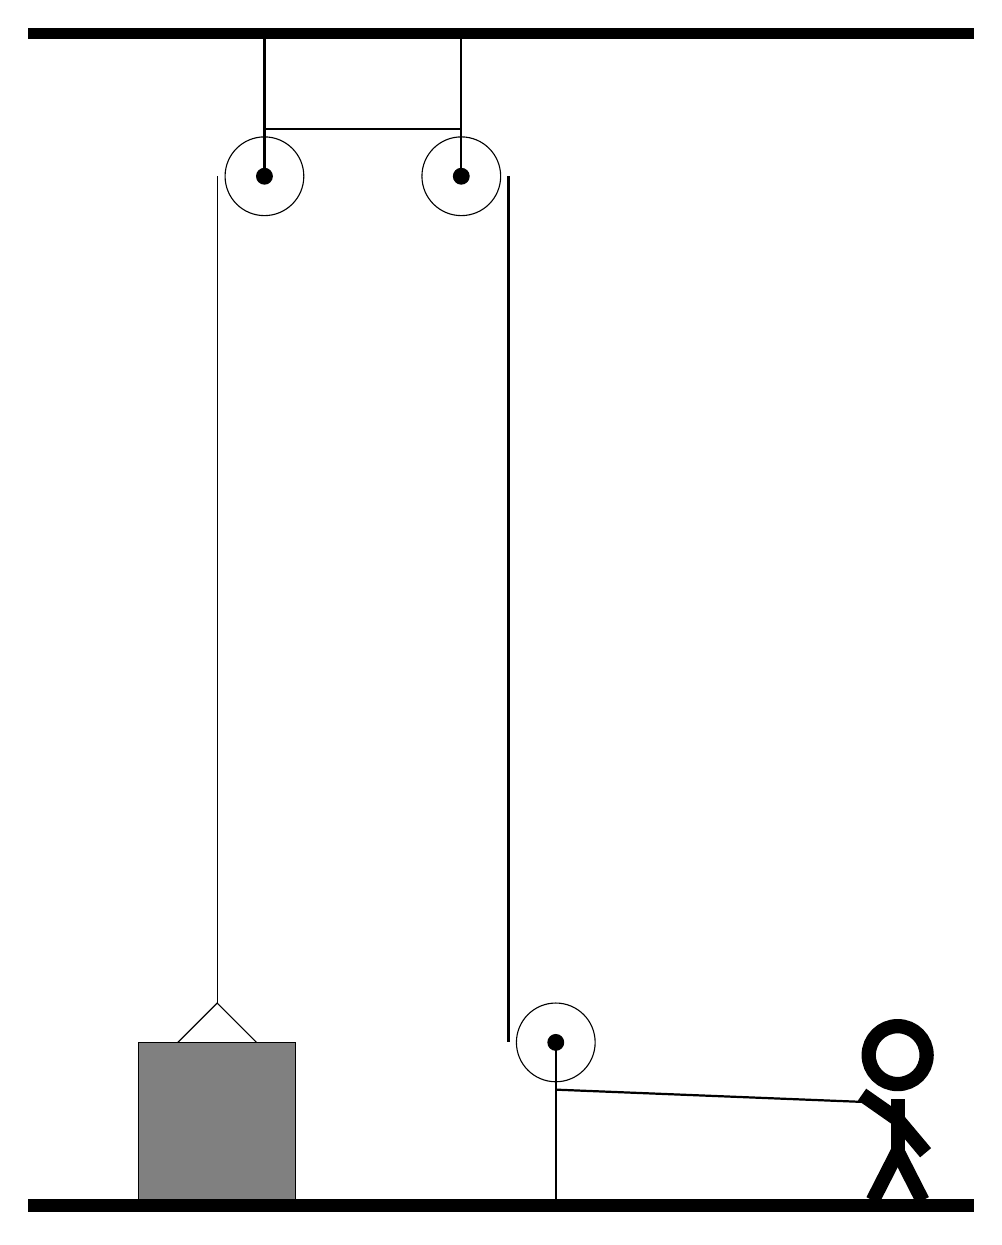
\begin{tikzpicture}
				%%%%% START %%%%%
								
				\draw[fill=black] (-2, 11.75) rectangle (10, 11.88);
				
				\draw (1, 10) circle (0.5);
				\draw[fill=black] (1, 10) circle (0.1);
				\draw[thick] (1, 11.75) -- (1, 10);
				
				\draw (3.5, 10) circle (0.5);
				\draw[fill=black] (3.5, 10) circle (0.1);
				\draw[thick] (3.5, 11.75) -- (3.5, 10);
				
				\draw (4.7, -1) circle (0.5);
				\draw[fill=black] (4.7, -1) circle (0.1);
				\draw[thick] (4.7, -3) -- (4.7, -1);
				
				\draw (-0.1, -1.0) --  (0.4, -0.5) -- (0.9, -1.0);
				\draw[fill=black!50] (-0.6, -1.0) rectangle (1.4, -3.0);
				
				\draw (0.4, 10) -- (0.4, -0.5);
				\centerarc[thick](1, 10)(90:180:0.6)
				\draw[thick] (1, 10.6) -- (3.5, 10.6);
				\centerarc[thick](3.5, 10)(0:90:0.6);
				\draw[thick](4.1, 10) -- (4.1, -1);
				\centerarc[thick](4.7, -1)(180:270:0.6);
				\draw[thick](4.7, -1.6) -- (8.7, -1.76);
				
				\node at (9, -1.9) {\Strichmaxerl[10][-35][-50]};
				
				\draw[fill=black] (-2, -3) rectangle (10, -3.15);
				%%%%% END %%%%%
			\end{tikzpicture}
	\end{figure}	
\end{document}